\chapter{Matrices}

\section{Matrix addition and scalar multiplication}

\begin{definition}
An $m\times n$ \emph{matrix} $A$ is a rectangular array with $m$ rows and $n$ columns; its
$(i,j)$-entry is written $a_{ij}$ or $(A)_{ij}$. The set of all $m\times n$ real matrices is
$\Mat{m}{n}$. Two matrices are equal if they have the same size and the same entries. Addition and
scalar multiplication are entrywise: $(A+B)_{ij}=a_{ij}+b_{ij}$, $(cA)_{ij}=ca_{ij}$. The
\emph{zero matrix} $O_{m,n}$ has all entries $0$.
\end{definition}

\begin{theorem}
$\Mat{m}{n}$ with these operations satisfies the same ten properties V1--V10 as $\R^n$ (with
$O_{m,n}$ playing the role of $\vec 0$).
\end{theorem}

\begin{definition}[Transpose]
The \emph{transpose} of an $m\times n$ matrix $A$ is the $n\times m$ matrix $A^T$ with
$(A^T)_{ij}=a_{ji}$: rows become columns. $A$ is \emph{symmetric} if $A^T=A$.
\end{definition}

\begin{theorem}
$(A^T)^T=A$, $(A+B)^T=A^T+B^T$, $(cA)^T=cA^T$.
\end{theorem}

\section{Matrix--vector multiplication}

We write $A=[\vec a_1\ \cdots\ \vec a_n]$ in terms of its columns $\vec a_j\in\R^m$.

\begin{definition}[Matrix--vector product]
For $A$ an $m\times n$ matrix and $\vec x\in\R^n$,
\[
  A\vec x = x_1\vec a_1 + x_2\vec a_2+\dots+x_n\vec a_n\in\R^m .
\]
\end{definition}

So $A\vec x$ is a linear combination of the columns of $A$ with weights from $\vec x$. Equivalently,
if $\vec r_1^T,\dots,\vec r_m^T$ are the rows of $A$, then the $i$-th entry of $A\vec x$ is the dot
product $\vec r_i\cdot\vec x$. The system of Chapter 3 is now compactly $A\vec x=\vec b$.

\begin{example}
\[
\begin{bmatrix} 1&2&0\\-1&3&1\end{bmatrix}\begin{bmatrix}2\\1\\-1\end{bmatrix}
= 2\begin{bmatrix}1\\-1\end{bmatrix}+1\begin{bmatrix}2\\3\end{bmatrix}-1\begin{bmatrix}0\\1\end{bmatrix}
=\begin{bmatrix}4\\0\end{bmatrix}.
\]
Row view: $(1,2,0)\cdot(2,1,-1)=4$ and $(-1,3,1)\cdot(2,1,-1)=-2+3-1=0$.
\end{example}

In the column view, $A\vec x$ is reached by walking $2$ copies of the first column, $1$ copy of
the second and $-1$ copy of the third:
\begin{center}
\begin{tikzpicture}[scale=0.75,>={Stealth}]
  \draw[very thin,gray!30] (-0.5,-2.5) grid (5.5,1.5);
  \draw[->] (-0.5,0) -- (5.8,0); \draw[->] (0,-2.5) -- (0,1.8);
  \draw[->,thick,blue!70!black] (0,0) -- (2,-2) node[midway,below left] {$2\vec a_1$};
  \draw[->,thick,green!50!black] (2,-2) -- (4,1) node[midway,left] {$1\vec a_2$};
  \draw[->,thick,orange!80!black] (4,1) -- (4,0) node[midway,right] {$-1\vec a_3$};
  \draw[->,very thick,red!70!black] (0,0) -- (4,0);
  \node[red!70!black,above] at (2.6,0) {$A\vec x = (4,0)$};
\end{tikzpicture}
\end{center}

\begin{theorem}[Linearity]
$A(\vec x+\vec y)=A\vec x+A\vec y$ and $A(c\vec x)=c(A\vec x)$. Also $A\vec e_j=\vec a_j$.
\end{theorem}

\begin{theorem}[Matrices Equal Theorem]
If $A$ and $B$ are $m\times n$ and $A\vec x=B\vec x$ for every $\vec x\in\R^n$, then $A=B$.
\end{theorem}
\begin{proof}
Take $\vec x=\vec e_j$: the $j$-th columns agree, $\vec a_j=A\vec e_j=B\vec e_j=\vec b_j$.
\end{proof}

\section{Matrix multiplication}

\begin{definition}[Matrix product]
For $A$ $m\times n$ and $B=[\vec b_1\ \cdots\ \vec b_p]$ $n\times p$, the product is the
$m\times p$ matrix
\[
  AB = [A\vec b_1\ \ A\vec b_2\ \cdots\ A\vec b_p], \qquad
  (AB)_{ij} = \sum_{k=1}^n a_{ik}b_{kj} = (\text{row } i \text{ of } A)\cdot(\text{column } j \text{ of } B).
\]
The product is defined only when the number of columns of $A$ equals the number of rows of $B$.
\end{definition}

\begin{center}
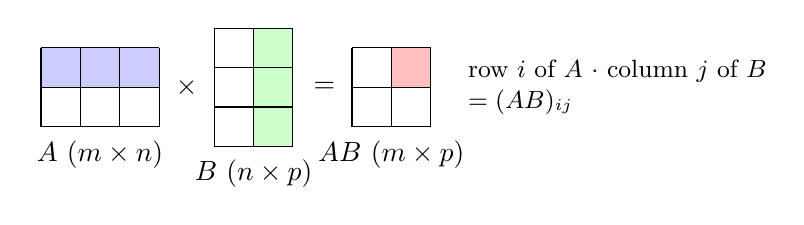
\begin{tikzpicture}[scale=0.5]
  % A: 2x3
  \draw (0,0) grid (3,2);
  \fill[blue!20] (0,1) rectangle (3,2); \draw (0,0) grid (3,2);
  \node at (1.5,-0.7) {$A$ ($m\times n$)};
  \node at (3.7,1) {$\times$};
  % B: 3x2
  \begin{scope}[xshift=4.4cm,yshift=-0.5cm]
    \fill[green!20] (1,0) rectangle (2,3); \draw (0,0) grid (2,3);
    \node at (1,-0.7) {$B$ ($n\times p$)};
  \end{scope}
  \node at (7.2,1) {$=$};
  \begin{scope}[xshift=7.9cm]
    \fill[red!25] (1,1) rectangle (2,2); \draw (0,0) grid (2,2);
    \node at (1,-0.7) {$AB$ ($m\times p$)};
  \end{scope}
  \node[right,font=\small,align=left] at (10.6,1) {row $i$ of $A$ $\cdot$ column $j$ of $B$\\ $= (AB)_{ij}$};
\end{tikzpicture}
\end{center}

The definition is chosen so that $(AB)\vec x = A(B\vec x)$: multiplying by $AB$ is the same as
first multiplying by $B$ then by $A$ (composition; Chapter 5).

\begin{example}
Let $A=\begin{bmatrix}1&2&0\\-1&3&1\end{bmatrix}$ and $B=\begin{bmatrix}2&1\\0&-1\\4&3\end{bmatrix}$. Then
\[
AB=\begin{bmatrix}1\cdot2+2\cdot0+0\cdot4 & 1\cdot1+2(-1)+0\cdot3\\
                  -1\cdot2+3\cdot0+1\cdot4 & -1\cdot1+3(-1)+1\cdot3\end{bmatrix}
  =\begin{bmatrix}2&-1\\2&-1\end{bmatrix},
\]
while $BA$ is $3\times3$:
\[
BA=\begin{bmatrix}2-1&4+3&0+1\\ 0+1&0-3&0-1\\ 4-3&8+9&0+3\end{bmatrix}
  =\begin{bmatrix}1&7&1\\1&-3&-1\\1&17&3\end{bmatrix}.
\]
\end{example}

\begin{theorem}[Properties of matrix multiplication]
Whenever the sizes make sense, and $c\in\R$:
\begin{enumerate}
  \item $A(B+C)=AB+AC$ and $(A+B)C=AC+BC$;
  \item $c(AB)=(cA)B=A(cB)$;
  \item $A(BC)=(AB)C$ (associativity);
  \item $(AB)^T=B^TA^T$.
\end{enumerate}
\end{theorem}
\begin{proof}[Proof of (3) and (4)]
(3): $\big(A(BC)\big)_{ij}=\sum_k a_{ik}\sum_l b_{kl}c_{lj}=\sum_l\big(\sum_k a_{ik}b_{kl}\big)c_{lj}
=\big((AB)C\big)_{ij}$.
(4): $((AB)^T)_{ij}=(AB)_{ji}=\sum_k a_{jk}b_{ki}=\sum_k (B^T)_{ik}(A^T)_{kj}=(B^TA^T)_{ij}$.
\end{proof}

\begin{important}[What does \emph{not} hold]
\begin{itemize}
  \item \textbf{Not commutative.} Even for square matrices, usually $AB\ne BA$:
  \[
  \begin{bmatrix}1&1\\0&1\end{bmatrix}\begin{bmatrix}1&0\\1&1\end{bmatrix}=\begin{bmatrix}2&1\\1&1\end{bmatrix},\qquad
  \begin{bmatrix}1&0\\1&1\end{bmatrix}\begin{bmatrix}1&1\\0&1\end{bmatrix}=\begin{bmatrix}1&1\\1&2\end{bmatrix}.
  \]
  Hence $(A+B)^2 = A^2+AB+BA+B^2$, \emph{not} $A^2+2AB+B^2$ in general.
  \item \textbf{No cancellation, zero divisors.} $AB=O$ does not imply $A=O$ or $B=O$:
  \[
  \begin{bmatrix}1&1\\1&1\end{bmatrix}\begin{bmatrix}1&-1\\-1&1\end{bmatrix}=\begin{bmatrix}0&0\\0&0\end{bmatrix}.
  \]
  Similarly $AB=AC$ does not imply $B=C$.
  \item The order reverses in $(AB)^T=B^TA^T$.
\end{itemize}
\end{important}

\section{The identity matrix and special matrices}

\begin{definition}
The $n\times n$ \emph{identity matrix} is $I_n=[\vec e_1\ \cdots\ \vec e_n]$, with $1$s on the
diagonal and $0$ elsewhere. A square matrix is \emph{upper triangular} if all entries below the
diagonal are $0$, \emph{lower triangular} if all entries above are $0$, and \emph{diagonal} if
both; we write $\diag(d_1,\dots,d_n)$.
\end{definition}

\begin{theorem}
For $A$ $m\times n$, $I_mA=A=AI_n$. Moreover $I_n$ is the \emph{unique} matrix with $I\vec x=\vec x$
for all $\vec x$.
\end{theorem}
\begin{proof}
$AI_n=[A\vec e_1\ \cdots\ A\vec e_n]=[\vec a_1\ \cdots\ \vec a_n]=A$. For $I_mA$, each column is
$I_m\vec a_j = \sum_i (\vec a_j)_i\vec e_i=\vec a_j$. Uniqueness follows from the Matrices Equal Theorem.
\end{proof}

Powers of a square matrix are defined by $A^0=I$, $A^{k+1}=A^kA$. Products of diagonal matrices
are easy: $\diag(a_1,\dots,a_n)\diag(b_1,\dots,b_n)=\diag(a_1b_1,\dots,a_nb_n)$, so
$\diag(d_1,\dots,d_n)^k=\diag(d_1^k,\dots,d_n^k)$. This is the key to Chapter 10.

\section{Block multiplication}

If matrices are partitioned into blocks of compatible sizes, they multiply ``as if the blocks
were numbers'' (keeping the order of factors). For example, if $A=[A_1\ A_2]$ (split by columns)
and $B=\begin{bmatrix}B_1\\B_2\end{bmatrix}$ (split by rows correspondingly), then $AB=A_1B_1+A_2B_2$.
A useful special case: the product of the column vector $\vec u\in\R^m$ with the row $\vec v^T$
($\vec v\in\R^n$) is the $m\times n$ \emph{outer product} $\vec u\vec v^T$, and
\[
  AB = \sum_{k=1}^n \vec a_k\vec b_k^{\,T} \quad(\vec a_k=\text{column } k \text{ of } A,\ \vec b_k^T=\text{row } k\text{ of } B).
\]
Note also that $\vec x\cdot\vec y = \vec x^T\vec y$ (a $1\times1$ matrix), which gives the useful
identity $(A\vec x)\cdot\vec y = \vec x\cdot(A^T\vec y)$.

\begin{proof}[Proof of the identity]
$(A\vec x)\cdot\vec y = (A\vec x)^T\vec y = \vec x^TA^T\vec y = \vec x\cdot(A^T\vec y)$.
\end{proof}

\section*{Summary}
\begin{itemize}
  \item $A\vec x=x_1\vec a_1+\dots+x_n\vec a_n$; entry $i$ is (row $i$)$\cdot\vec x$.
  \item $AB=[A\vec b_1\cdots A\vec b_p]$, $(AB)_{ij}=\sum_k a_{ik}b_{kj}$; defined when inner sizes match.
  \item Associative and distributive, $(AB)^T=B^TA^T$; \emph{not} commutative and no cancellation.
  \item $A\vec x=B\vec x$ for all $\vec x$ implies $A=B$. $I$ is the multiplicative identity.
\end{itemize}
